\thechapter{Experimental results} 

\begin{wrapfigure}{r}{0.5\textwidth}
\centering
\begin{subfigure}[b]{0.28\textwidth}
        
\includegraphics[width=\textwidth]{img/Textures/TextureLightingCelShade.png}
\end{subfigure}
\caption{Cel Shaded Texture Final}
 \label{fig:TextureLightingCelShade}
\end{wrapfigure} 

Our system was able to produce the best results using models with higher vertex counts and smooth curves like the skull, while the engineer was more problematic, but increasing the vertex count also significantly increased the time to produce the render. Many aspects needed to be customized to particular models to get optimal results.

When our simple Cel Shading algorithm is applied to some textures the colours output need correction especially at lower levels as in \ref{fig:CelShadeTexture4}, but combined with cel shaded lighting using more levels for the texture the desired effect can be produced \ref{fig:CelShadeTexture4}. 

%\begin{wrapfigure}{r}{0.5\textwidth}
\begin{figure}[h]
\centering
\begin{subfigure}[b]{0.18\textwidth}
        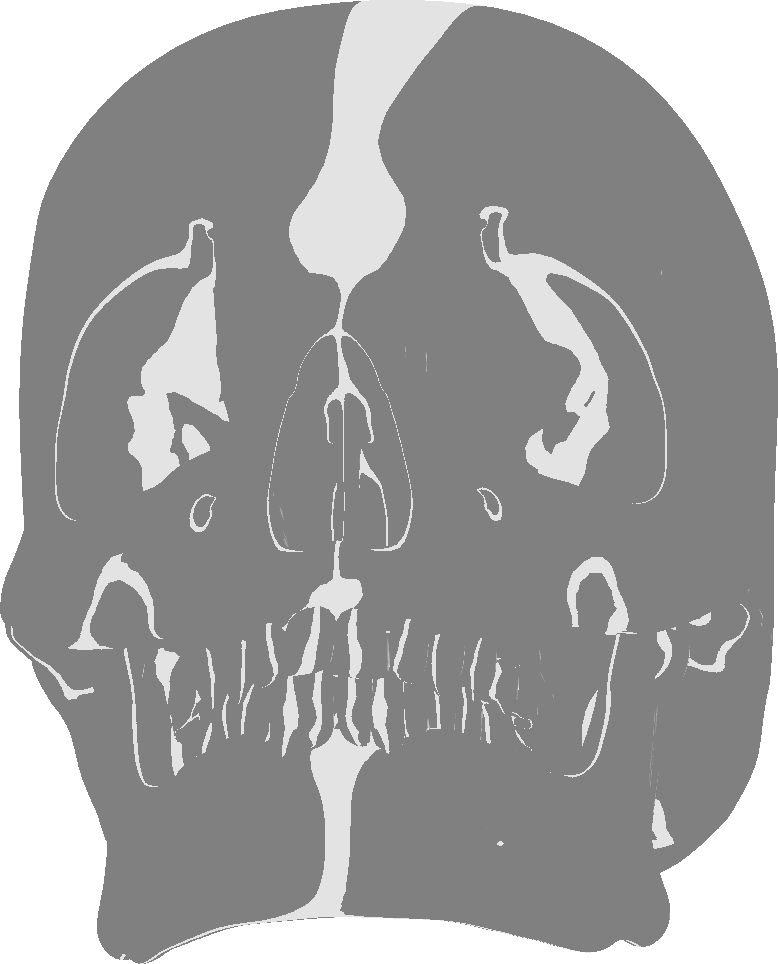
\includegraphics[width=\textwidth]{img/Lighting/Directional.png}
        \caption{Directional}
        \label{fig:LightingPosDir}
\end{subfigure}
    ~
    \begin{subfigure}[b]{0.18\textwidth}
        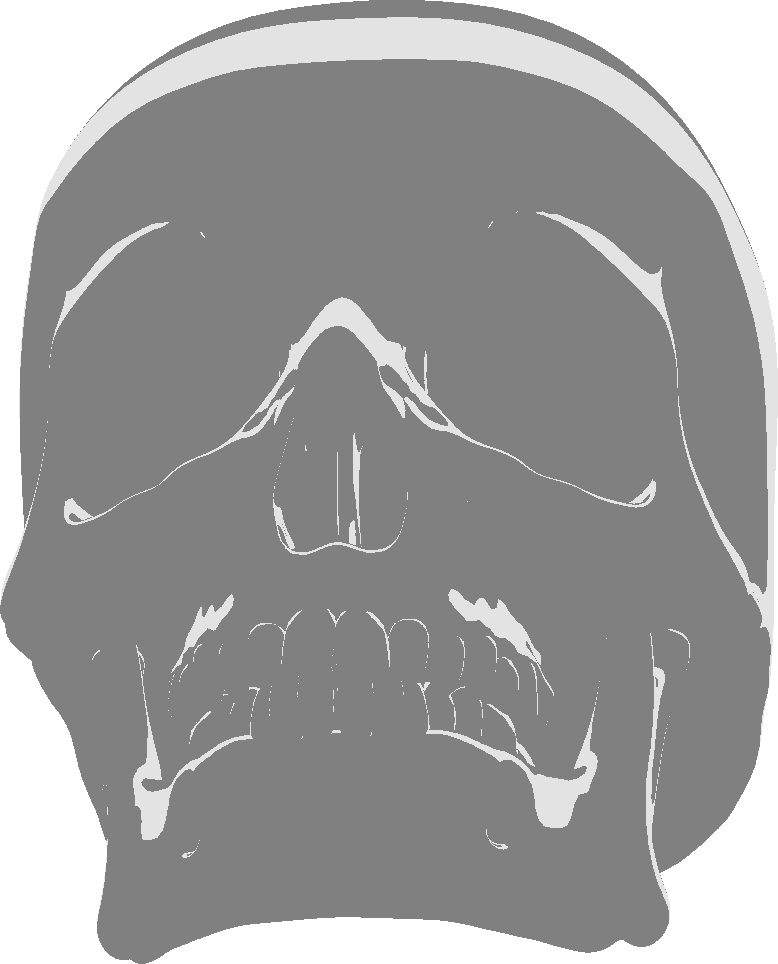
\includegraphics[width=\textwidth]{img/Lighting/Point.png}
        \caption{Point}
        \label{fig:LightingPosPos}
    \end{subfigure}
\caption{Rim Lighting and Light Position}
 \label{fig:LightingPosRim}
 \end{figure}
%\end{wrapfigure} 

Positioning of the light for optimally rending the lighting is highly dependant on the model, and the area of the model that is being viewed. Depending on the positioning of the lighting the effect can vary greatly, demonstrated in \ref{fig:LightingPosRim} where the rim lighting on the model appears dramatically different depending on the distance away it is.

